\documentclass[12pt]{article}
\usepackage{geometry}
\geometry{ b4paper, total={220mm,320mm}, left=20mm,
            top=15mm, headheight=33pt,includeheadfoot}

\usepackage[parfill]{parskip}  % Activate to begin paragraphs with an empty line rather than an indent
\usepackage{graphicx}

\usepackage{mathtools}
\usepackage{blindtext}
\usepackage{multicol}
\usepackage{listings, matlab-prettifier}
\usepackage{tikz, circuitikz}
\usepackage{wrapfig}
\usepackage{longtable}
\usepackage{booktabs, caption, colortbl}
\usepackage{pdflscape}
\usepackage{appendix}

\usepackage{pgfplots}
\pgfplotsset{
    compat=1.18,
    label style={font=\tiny\sffamily},
    % legend style={font=\footnotesize},
    % title style={font=\scriptsize}
    no markers,
    every axis plot/.append style={thin},
    every tick label/.append style={font=\tiny\sffamily},
    grid=both,
    tick align=outside,
    tickpos=left,
    grid style={line width=.1pt, draw=gray!10},
    major grid style={line width=.2pt,draw=gray!50},
    minor tick num=3,
    %enlargelimits={abs=0.5},
    axis line style={latex-latex}
}

\usepackage{amssymb}
\usepackage{enumitem}
\usepackage{amsmath}

\usepackage{fancyhdr, lastpage, setspace}
\pagestyle{fancy}
\usepackage{caption, subcaption, zref-totpages}

\usepackage{fontspec}
\usepackage{microtype}

\usepackage{polyglossia}

\usepackage[dvipsnames]{xcolor} %red, green, blue, yellow, cyan, magenta, black, white

%\def\pdfpageref{\pdffeedback pageref}
\usepackage{hyperref}
\hypersetup{
    bookmarksopen=true,
    colorlinks=true,
    linkcolor=black,
    filecolor=magenta,      
    urlcolor=black,
    pdftitle={Parametric Study of a Microwave Absorver Based on Metamaterials}
}

\setmainlanguage{english}
\setdefaultlanguage{english}
\setotherlanguages{greek}

\usepackage[ backend=biber, bibencoding=utf8, style=ieee]{biblatex}
\addbibresource{ref.bib}

\listfiles

\urlstyle{same}

\rhead{
\includegraphics[width=1cm]{ece.png}}
\lhead{
\includegraphics[height=1cm]{uowm.png}}

\fancyfoot{}
\fancyfoot[RO]{\thepage /\ztotpages}

\graphicspath{ {img} }
%\addmediapath{ {video} }

\setmainfont[Ligatures=TeX,Numbers=Lining]{Linux Libertine}
\setsansfont[Kerning=On]{Atkinson Hyperlegible}
\setmonofont{Corbel}

\renewcommand{\thesection}{\Roman{section}}
\renewcommand{\thesubsection}{\thesection.\Roman{subsection}}
\renewcommand{\thesubsubsection}{\thesubsection.\Roman{subsubsection}}

\newcommand{\ra}[1]{\renewcommand{\arraystretch}{#1}}

\onehalfspacing

\AddToHook{env/landscape/begin}
 {%
  \clearpage
  \pagestyle{empty}
  \AddToHook{shipout/background}[sven/page]
    {
     \put(0.9\paperwidth,-0.5\paperheight)%adapt values
      {\rotatebox{90}{\thepage}}
    }%
 }     

\AddToHook{env/landscape/after}
 {\RemoveFromHook{shipout/background}[sven/page]}

\title{ \textsf{Parametric Study of a Microwave Absorber Based on Metamaterials.}\\
    %\textsf{Special Project}\\
    \textsf{\Large Department of Electrical \& Computer Engineering}\\
    \textsf{\large University of Western Macedonia}
} \author{\textsf{Markos Delaportas} \footnote{E-mail: ece01316@uowm.gr}}
\date{\textsf{March 2025}}

\begin{document}

\maketitle

\textbf{ \textit{Abstract} -- Microwave absorbers play a crucial role in modern
    telecommunications and electronic systems by mitigating unwanted electromagnetic
    interference (EMI) and enhancing the performance of various devices. These absorbers are
    essential in applications ranging from radar systems and anechoic chambers to consumer
    electronics and medical devices. Traditional microwave absorbers, while effective, often
    suffer from limitations such as bulkiness and narrow bandwidth. Metamaterial-based
    microwave absorbers offer a promising alternative due to their unique electromagnetic
    properties, which are not found in natural materials. These engineered materials can
    achieve near-unity absorption across a wide range of frequencies, making them highly
    efficient. The advantages of metamaterial absorbers include their thin profile,
    lightweight nature, and the ability to tailor their absorption characteristics through
    precise structural design. This makes them ideal for applications requiring compact and
    efficient EMI mitigation. Additionally, metamaterial absorbers can be designed to operate
    over multiple frequency bands, providing versatility and enhanced performance in complex
    electromagnetic environments.}

{\let\clearpage\relax \tableofcontents} \thispagestyle{empty}    
%\tableofcontents


\section{\textsf{Introduction}}
    Metamaterials are artificially designed materials that
    exhibit peculiar properties like negative refractive index \cite{veselago_left_2006}, 
    Snell's law reversal \cite{wang_simulationguided_2024}, Doppler effect reverse
    \cite{jha_design_2018}, and left-handed behavior. These properties make them suitable
    for various applications, including perfect absorption. Metamaterial absorbers can
    achieve near-unity absorption, thin profiles, lightweight characteristics, and design
    flexibility.

    The development of metamaterial absorbers has seen significant progress, with
    researchers exploring various designs and materials to enhance their performance.
    Metamaterial absorbers are predominantly used in the microwave, terahertz, and optical
    frequency spectra. Recent advancements include the development of multi-band
    polarization-insensitive metamaterial absorbers for microwave applications, broadband
    microwave coding metamaterial absorbers \cite{tran_broadband_2020}, and ultra-wideband
    origami microwave absorbers\cite{biswas_ultra-wideband_2022}.

    This study begins with a theoretical exploration of absorber devices and the unique
    properties of metamaterials that make them suitable for electromagnetic wave absorption.
    Following this, the report details the implementation of a specific microwave absorber
    device using advanced simulation software, highlighting the practical aspects of device
    design and performance evaluation. Finally, the report addresses the parametric design and
    optimization of the device, fine-tuning structural parameters to achieve optimal absorption
    characteristics. Through this comprehensive approach, the report aims to provide a thorough
    understanding of the principles, design methodologies, and practical applications of
    metamaterial-based microwave absorbers.

\section{\textsf{Theoretical Study}}
    Metamaterials are artificially engineered materials with unique electromagnetic properties
    not found in nature. They are designed with specific geometrical structures that allow them
    to exhibit properties like negative refractive index, reverse Snell's law, and right/left-handed
    behavior. 
    
    An MMA typically comprises three layers: 
    \begin{itemize}
        \item A periodic metallic pattern on top
        \item A dielectric substrate in the middle
        \item A bottom metallic ground plane
    \end{itemize}
    This layered structure enables efficient absorption of electromagnetic waves.

    Impedance matching is crucial for MMAs to minimize reflection and maximize absorption. 
    This is achieved when the impedance of the MMA is matched to the impedance of free space,
    ensuring that incident electromagnetic waves are absorbed rather than reflected.
    
    Reducing the plasma frequency of metals in MMAs allows them to operate effectively at 
    lower frequencies, expanding their applicability to various frequency ranges. 
    This is achieved by manipulating the density of free electron carriers in the metal.

    Multi-layer structures in MMAs enable broadband absorption by creating multiple resonant
    frequencies. By stacking different layers with varying properties, a wider range of 
    frequencies can be absorbed effectively.


    Designing MMAs for specific applications often presents challenges related to achieving 
    the desired bandwidth and absorption ratio. Balancing these requirements while considering
    factors like size, complexity, and cost can be difficult, requiring careful optimization
    of the MMA structure and materials.

    \subsection{\textsf{Impedance Matching Free Space}}
        An absorber can be represented as a transmission line equivalent
        \cite{biswas_ultra-wideband_2022}. In order to maximize the absorbance\dots 

    \subsection{\textsf{Magnetic Resonance}}
        Is what can be achieved with closed loop structures \cite{abdulkarim_review_2022}.
    
    \subsection{\textsf{Electrical Resonance}}
        Can be achieved introducing gaps in the structure \cite{abdulkarim_review_2022}.

    \subsection{\textsf{Plasma Frequency}}
        Plasma frequency of a material is the electron cloud oscillations for a specific material.
        \begin{equation}
            \omega_p = \sqrt{\frac{Ne^2}{m\epsilon_0}}
        \end{equation} 
\section{\textsf{Simulation}} 
    The simulation was conducted using CST (Computer Simulation Technology)
    software to implement a configuration inspired by the design presented 
    in \cite{zhang_design_2023}. This section outlines the steps taken to 
    model the structure, the assumptions made, and the results obtained from
    the simulation.

    \subsection{\textsf{CST Implementation}} 
        The vertical layout in CST consists of a three-layer structure:
        \begin{itemize}
        \item \textbf{Dielectric Substrate}:  This layer serves as the 
            base for the structure.
        \item \textbf{Air Gap}: Positioned above the dielectric substrate,
            this layer introduces an air gap to influence the electromagnetic 
            properties.
        \item \textbf{Metal Backplate}: The top layer, made of copper, 
            acts as a reflective surface.
        \end{itemize}

        The dielectric substrate also includes a metallic component, which
        is made of the same material as the metal backplate—copper, with
        a conductivity of (5.96 \mu $10^7$ S/m).

        Initially, the FR-4 substrate is placed without the metal 
        resonance layer. The other two layers are positioned below $Z=0$. 
        When viewed from the orthographic side, the layout appears as shown
        in Figure (\ref{img:layout}).
        \begin{figure}[h]
            \centering
            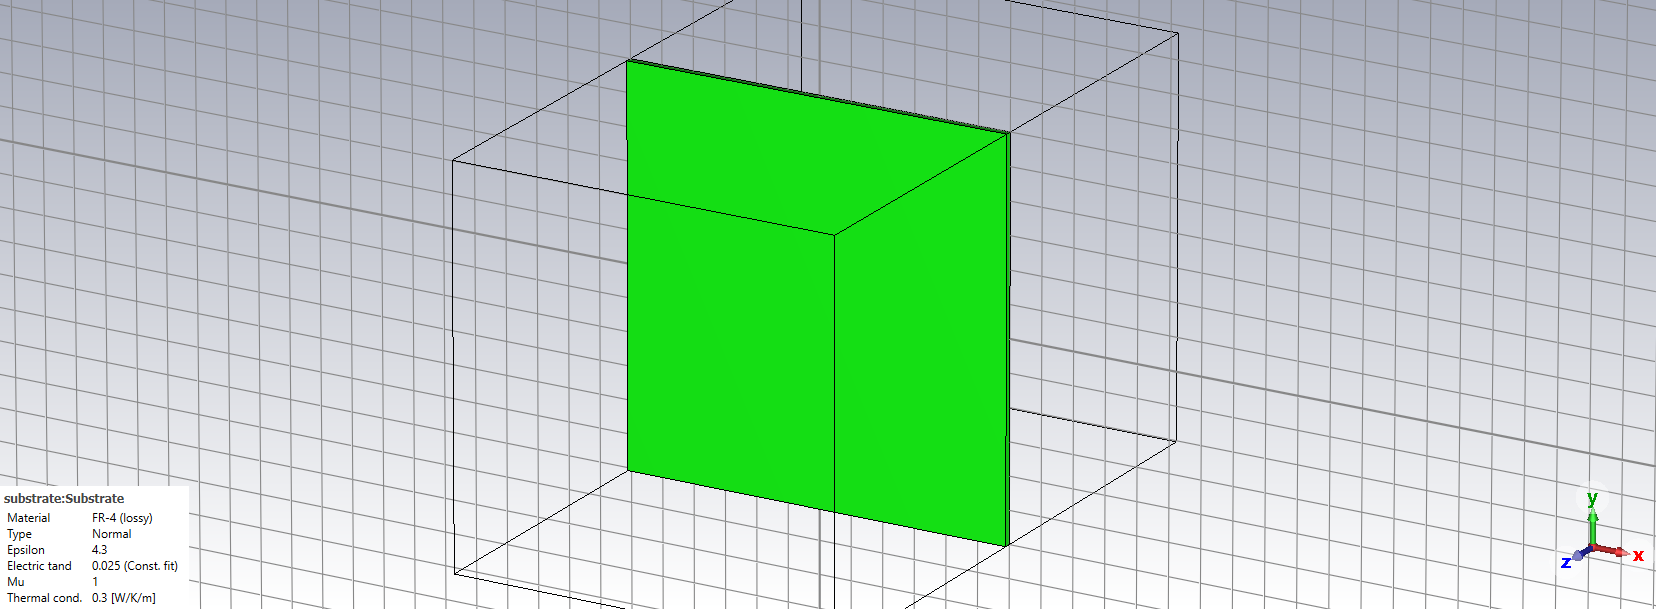
\includegraphics[width=0.4\textwidth]{substrate.png}\hfil
            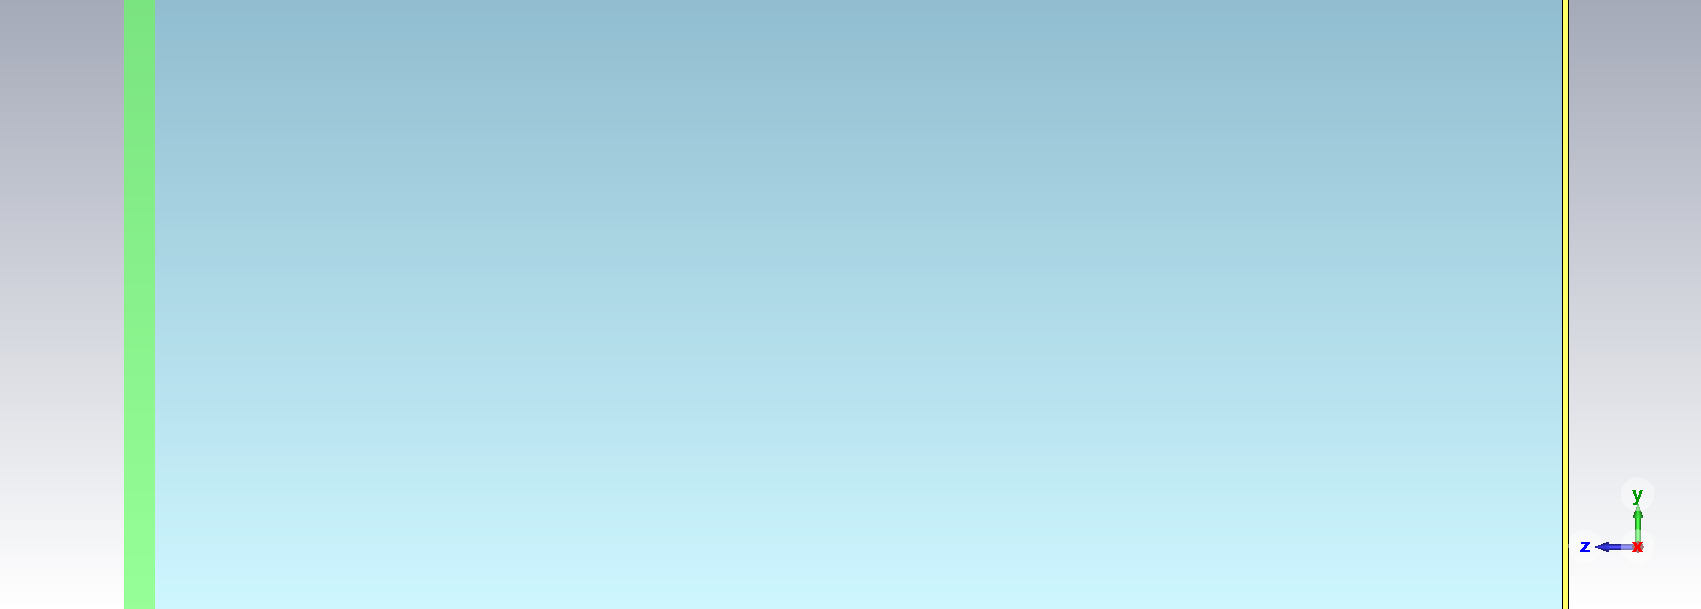
\includegraphics[width=0.4\textwidth]{verticaLayout.png}
            \caption{Basic Vertical Layout}
            \label{img:layout}
        \end{figure}

        Next, a ring resonator is added on top of the dielectric substrate. 
        The ring is made of the same material and thickness as the backplate, 
        as illustrated in Figure (\ref{img:ring}).
        \begin{figure}[h]
            \centering
            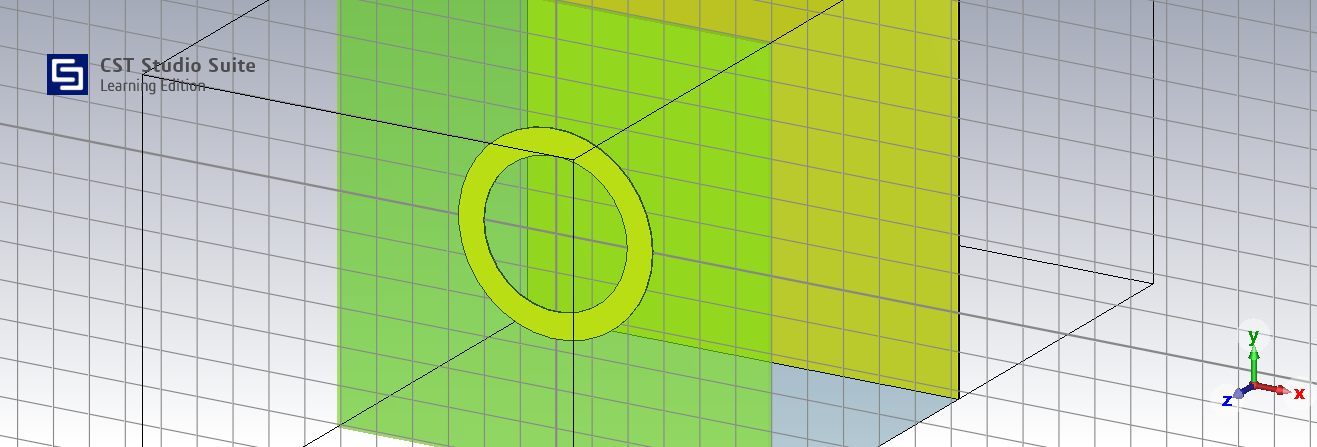
\includegraphics[width=0.6\textwidth]{ring.png}
            \caption{Ring Resonator}
            \label{img:ring}
        \end{figure}

        An important assumption in this design is that both the body and the 
        tip of the arrow have a width of $\alpha=0.5 mm$. To accurately place
        the curve points defining the arrow, a system of equations must be 
        solved to determine the Cartesian coordinates of the arrow's base points. 
        These points lie on the arc of the ring and are equidistant from the curve 
        $y=x$. The following MATLAB code snippet demonstrates the solution to this 
        system:
        \begin{lstlisting}[frame=single, numbers=left, style=Matlab-Pyglike]
            syms x1 x2

            eq1 = 2*(x1 - x2)^2 == .5^2; eq2 = sqrt(x2^2 + x1^2) == 2.7;

            sol = solve([eq1, eq2], [x1 x2]); disp([sol.x1 sol.x2]);  
        \end{lstlisting}
        
        This system simplifies to the equations shown in Equation (\ref{eq:xysys}).
        \begin{equation}
            \label{eq:xysys}
            \displaystyle \begin{array}{l} 
                \left(\begin{array}{cc} 
                    \sigma_3 -\frac{2916\,\sigma_1 }{1433} & -\sigma_1 \\
                    \sigma_4 -\frac{2916\,\sigma_2 }{1433} & -\sigma_2 \\
                    \frac{2916\,\sigma_1 }{1433}-\sigma_3  & \sigma_1 \\
                    \frac{2916\,\sigma_2 }{1433}-\sigma_4  & \sigma_2  
                \end{array}\right)\\
                \mathrm{}\\
                \textrm{where}\\
                \mathrm{}\\
                \;\;\sigma_1 =\sqrt{\frac{729}{200}-\frac{7\,\sqrt{59}}{80}}\\
                \mathrm{}\\
                \;\;\sigma_2 =\sqrt{\frac{7\,\sqrt{59}}{80}+\frac{729}{200}}\\
                \mathrm{}\\
                \;\;\sigma_3 =\frac{400\,{{\left(\frac{729}{200}-\frac{7\,\sqrt{59}}{80}\right)}}^{3/2} }{1433}\\
                \mathrm{}\\
                \;\;\sigma_4 =\frac{400\,{{\left(\frac{7\,\sqrt{59}}{80}+\frac{729}{200}\right)}}^{3/2} }{1433}
            \end{array}
        \end{equation}

        The arrow is then mirrored across the X, Y, and XY planes to cover all
        four sides of the cell. The face is covered with copper, and a height of 
        $d=0.035 mm$ is assigned, as shown in Figure (\ref{img:mirrorAndCover}).
        This step is crucial because all other layers were initially positioned 
        below $Z=0$.
        \begin{figure}[h]
            \centering
            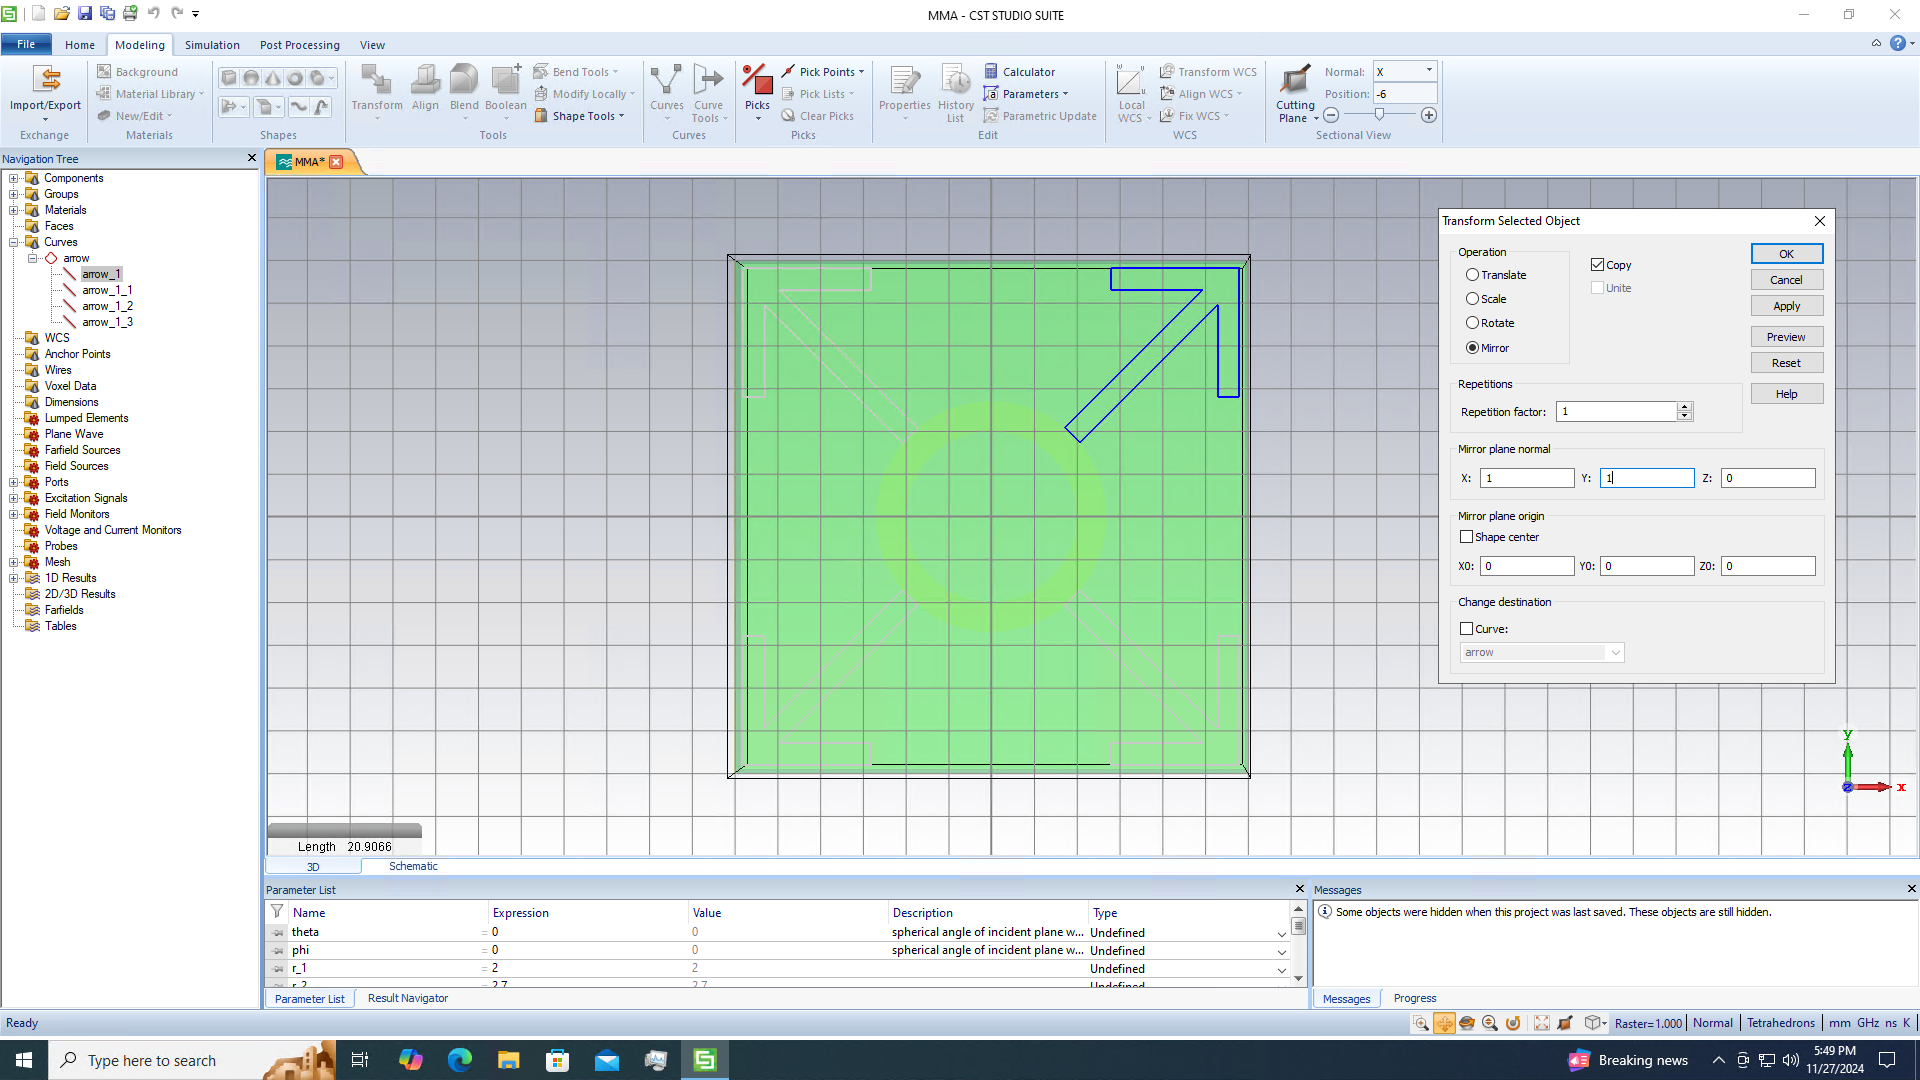
\includegraphics[width=.4\textwidth]{mirroredArrows.png}\hfil
            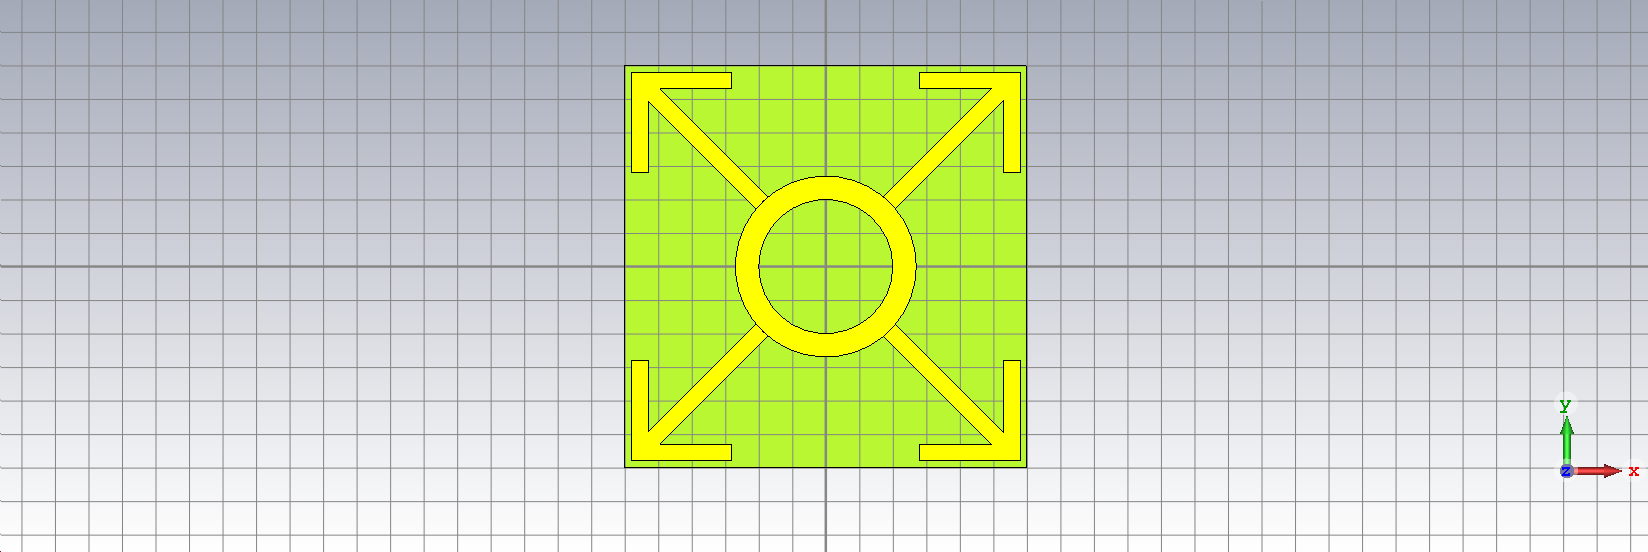
\includegraphics[width=.4\textwidth]{RingAndArrows.png}
            \caption{Mirroring Arrow and Cover}
            \label{img:mirrorAndCover}
        \end{figure}

        A series of cuts (boolean subtractions) are made in the resonance layer
        to add resistors between the copper faces near the arrows, as depicted 
        in Figure (\ref{img:arrowCuts}).
        \begin{figure}[h]
            \centering
            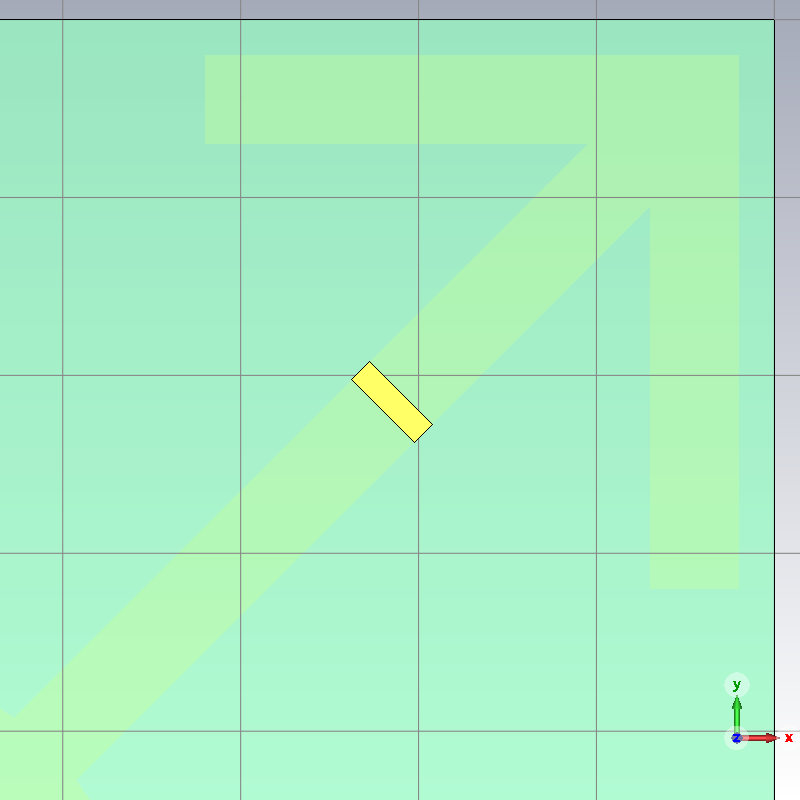
\includegraphics[width=.4\textwidth]{subtract.png}\hfil
            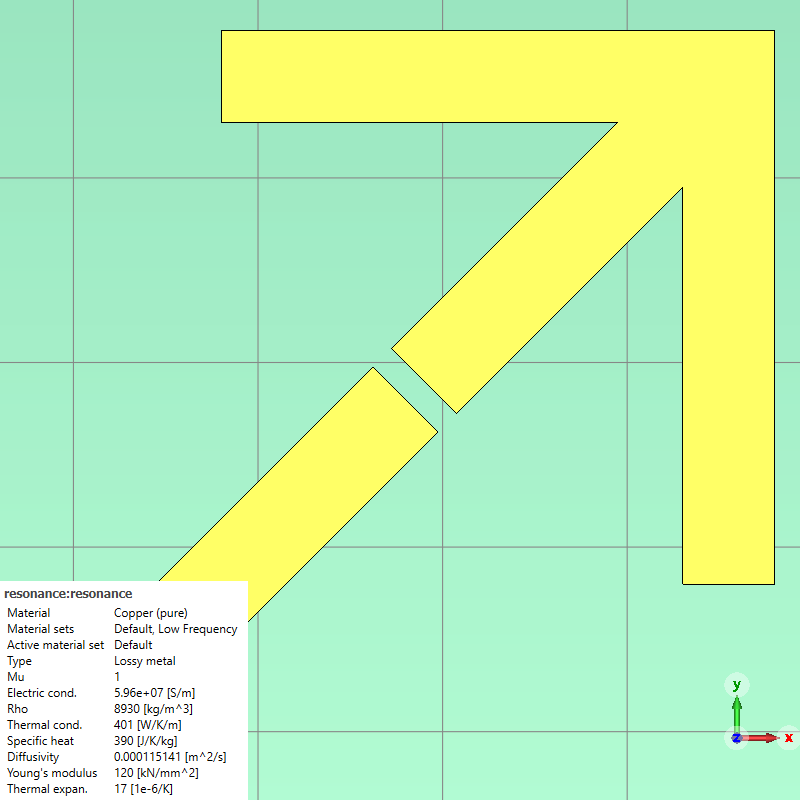
\includegraphics[width=.4\textwidth]{subtracted.png}
            \caption{Cuts Near the Arrows}
            \label{img:arrowCuts}
        \end{figure}

        Similar cuts are made near the ring to ensure uniform width, as shown 
        in Figure (\ref{img:ringCuts}).
        \begin{figure}[h]
            \centering
            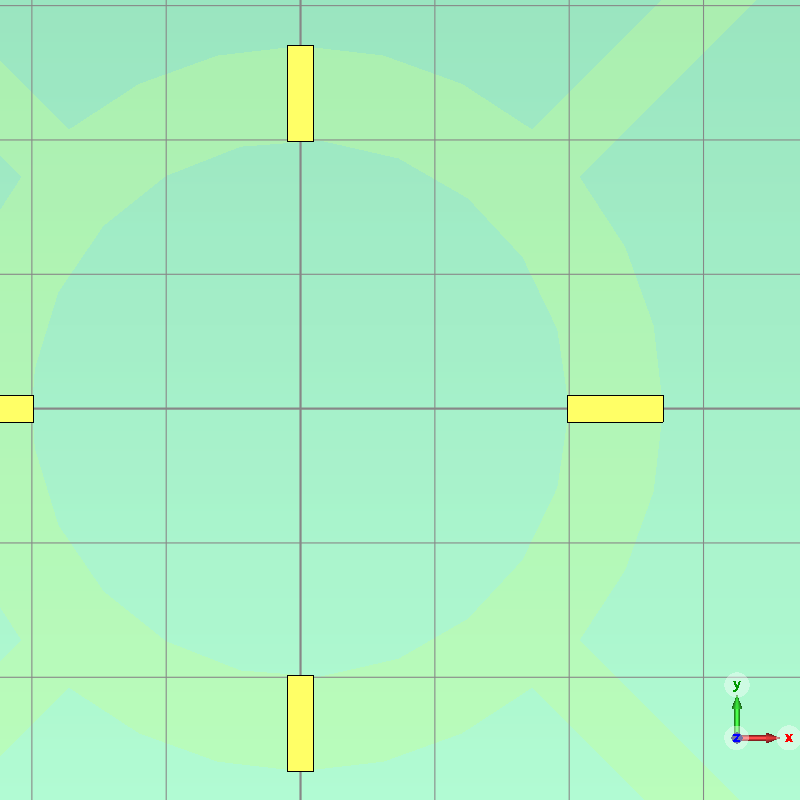
\includegraphics[width=.4\textwidth]{subtractRing.png}\hfil
            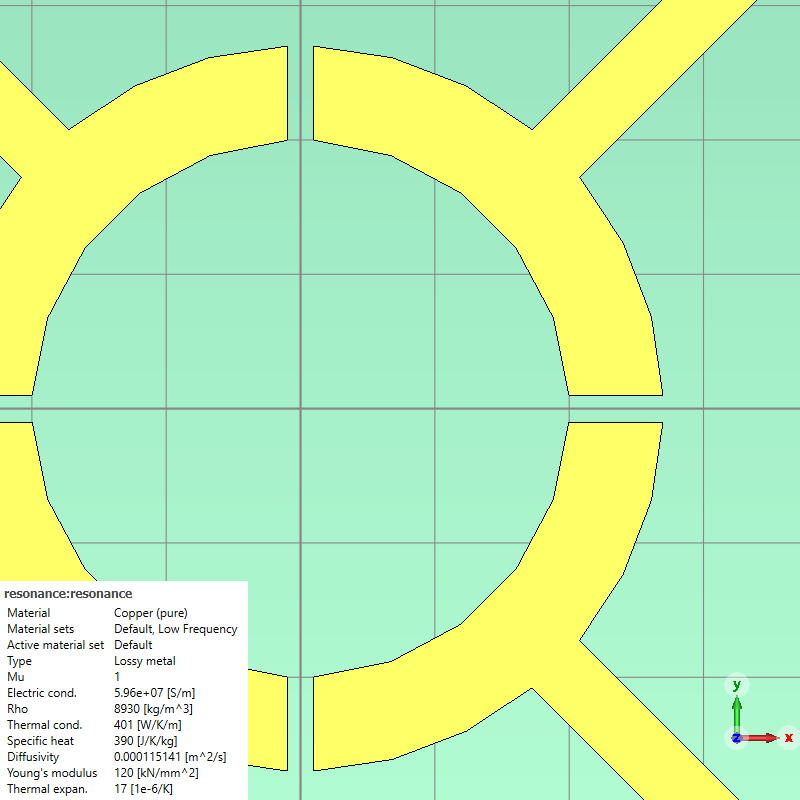
\includegraphics[width=.4\textwidth]{subtractedRing.png}
            \caption{Cuts Near the Ring}
            \label{img:ringCuts}
        \end{figure}

        Resistors are then added, connecting to the center points of the faces
        created by the previous subtractions, as illustrated in Figure 
        (\ref{img:resistors}). It is important to note that the performance of 
        the absorber may be reduced in this implementation. Better absorbance 
        might be achieved if the connection height is set to $d=0.035mm$.

        To perform the simulation using the frequency solver in CST, periodic 
        boundaries are set along the XY plane, and free space conditions are 
        applied along the Z axis. The resulting mesh is shown in Figure 
        (\ref{img:RingAndArrowMesh}).
        
        \begin{figure}
            \centering
            \begin{subfigure}{0.49\textwidth}
                \centering
                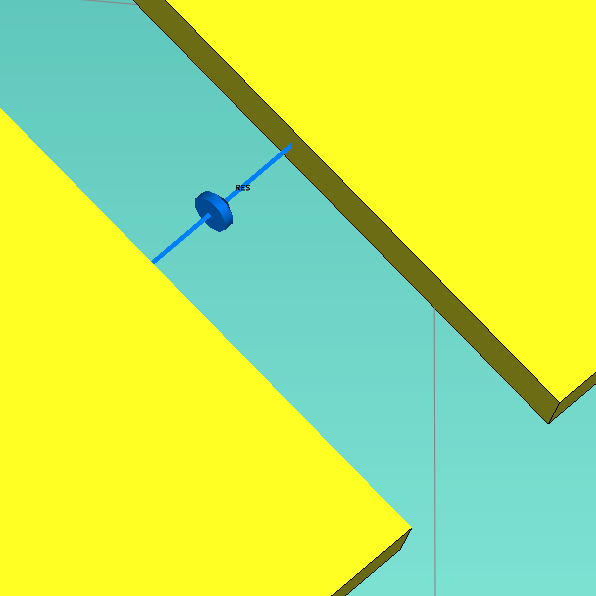
\includegraphics[width=\textwidth]{faceCenterPoint.png}
                \caption{Resistor Placement}
                \label{img:resistors}
            \end{subfigure}
            \hfill
            \begin{subfigure}{0.49\textwidth}
                \centering
                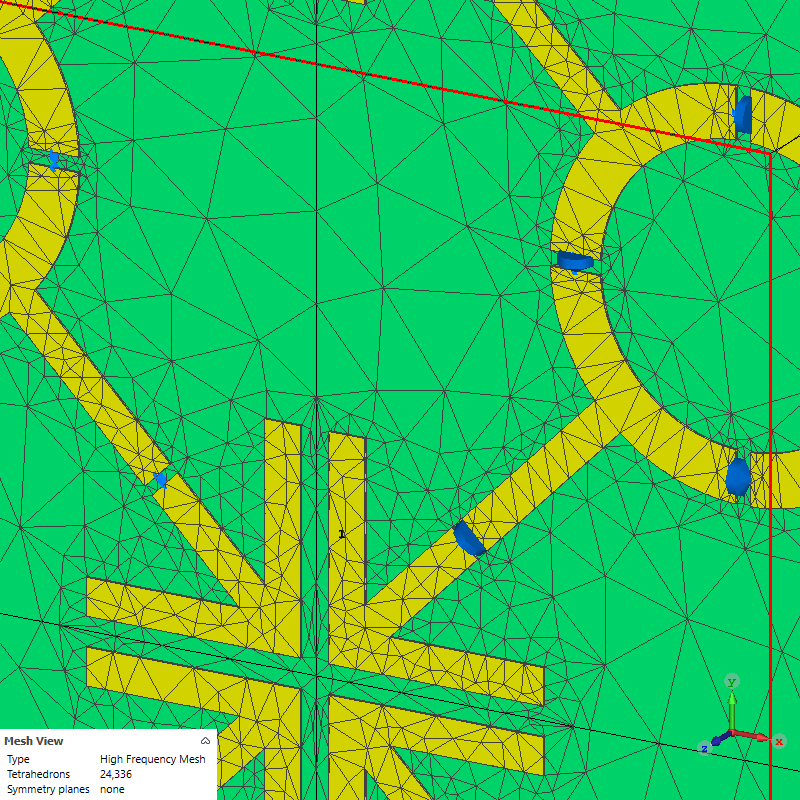
\includegraphics[width=\textwidth]{mesh.png}
                \caption{Ring Mesh for reference}
                \label{img:RingAndArrowMesh}
            \end{subfigure}
            \caption{Mesh around Resistors}
            \label{fig:combined}
        \end{figure}

        The electrical field absorbance is analyzed at different frequencies. 
        Figure (\ref{img:E_Zmax1}) shows the electrical field for $Z_{max}(1)$
        at frequencies of 2.7 GHz, 7.7 GHz, and 12.7 GHz.
        \begin{figure}[h]
            \centering
            
            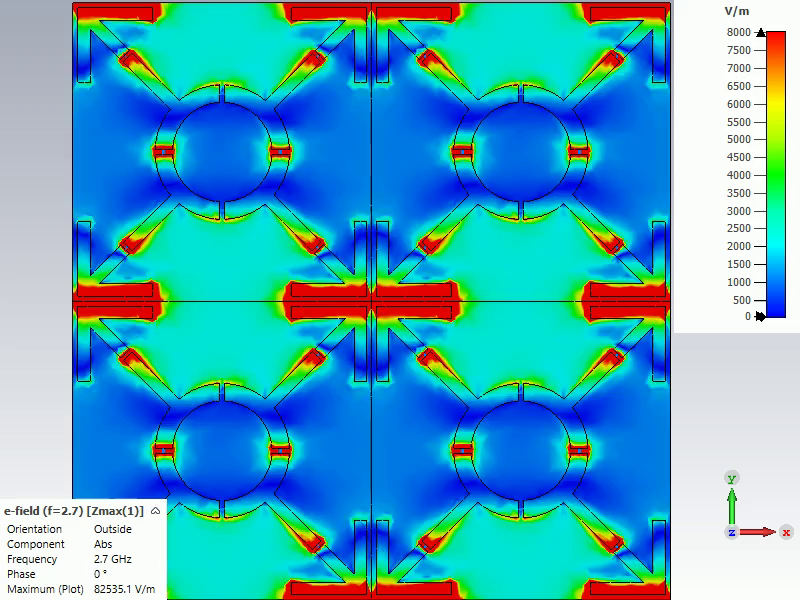
\includegraphics[page=1, width=0.22\textwidth]{E_Zmax1_027e2MHz.png}\hfil
            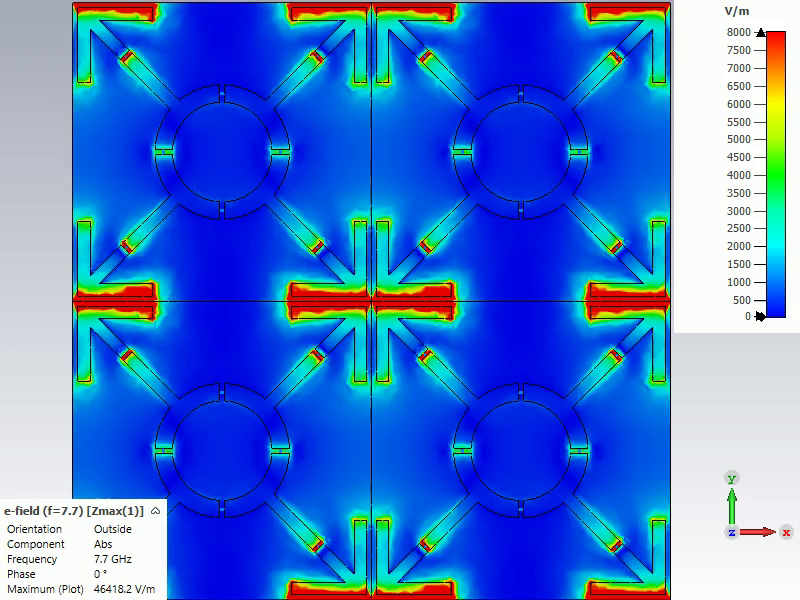
\includegraphics[page=1, width=0.22\textwidth]{E_Zmax1_077e2MHz.png}\hfil
            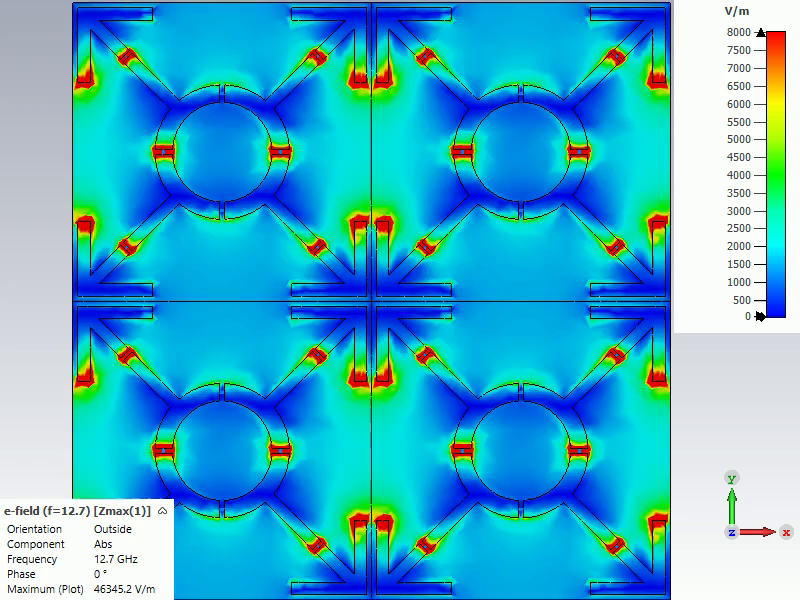
\includegraphics[page=1, width=0.22\textwidth]{E_Zmax1_127e2MHz.png}
            
            \caption{Electrical Field for [2.7, 7.7, 12.7] GHz $Z_{max}(1)$}
            \label{img:E_Zmax1}
        \end{figure}

        Similarly, Figure (\ref{img:E_Zmax2}) shows the electrical field for $Z_{max}(2)$
        at the same frequencies.
        \begin{figure}[h]
            \centering
            
            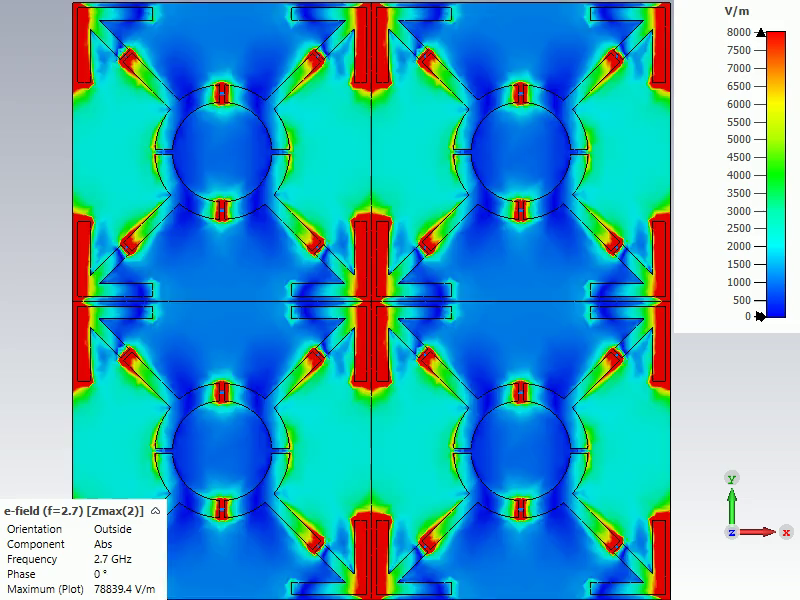
\includegraphics[page=1, width=0.22\textwidth]{E_Zmax2_027e2MHz.png}\hfil
            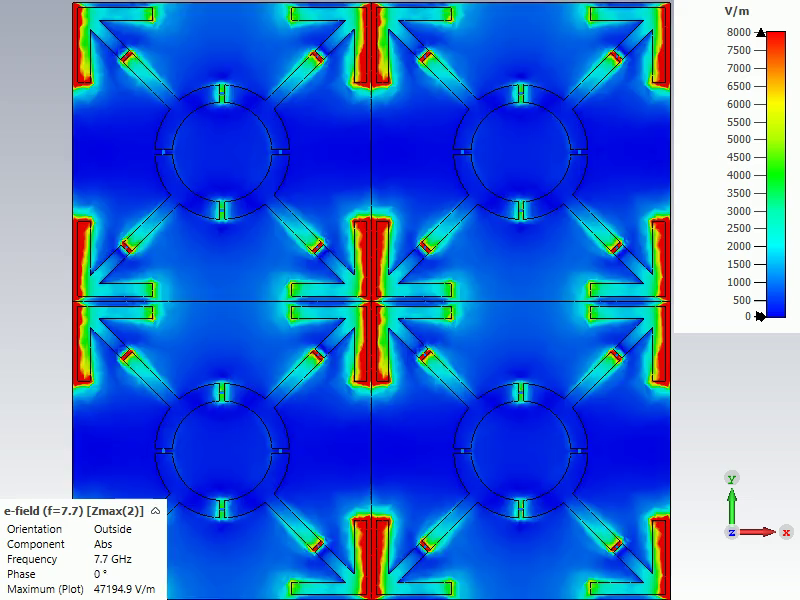
\includegraphics[page=1, width=0.22\textwidth]{E_Zmax2_077e2MHz.png}\hfil
            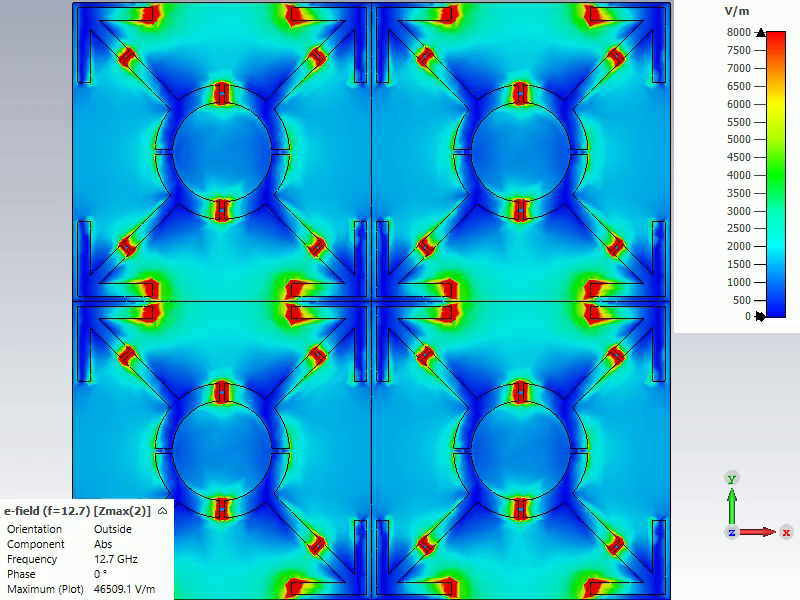
\includegraphics[page=1, width=0.22\textwidth]{E_Zmax2_127e2MHz.png}
            
            \caption{Electrical Field for [2.7, 7.7, 12.7] GHz $Z_{max}(2)$}
            \label{img:E_Zmax2}
        \end{figure}

        Taking a look in the $S_{11}$ of $Z_{max}$ after the simulation as such
        (\ref{plt:S11_Zmax}). The Absorptivity (against the frequency) is an
        essential metric and CST calculates it as shown in (\ref{plt:Absorptivity}).
        For the evaluation of the absorber Absorptivity can be calculated using the
        formula: $ A = 1 - |S_{11}|^2 - |T|^2 $, where T is the transmission
        coefficient and can be calculated using the formula: $T =
        \frac{2Z_0}{Z+Z_0}$. However the $Z$ mentioned needs to be the normalized
        impedance of the absorber so this is where the calculation will start.

        \begin{center}
            \begin{minipage}{.45\textwidth}
                \begin{tikzpicture}
                    \begin{axis}[ 
                        title={\textsf{Reflection Coefficient}},
                        xlabel={Frequency (GHz)}, ylabel={$S_{11}$ (dB)} 
                    ] \addplot table[x=freq, y=s11, col sep=space] {data/s11.txt};
                    \end{axis}
                \end{tikzpicture}
                %\captionof{figure}{\textsf{The $S_{11}$}}
                \label{plt:S11_Zmax}
            \end{minipage}
            \begin{minipage}{.45\textwidth}
                \begin{tikzpicture}
                    \begin{axis}[ 
                        title={\textsf{A/\small\lambda}},
                        xlabel={Wavelength (\lambda)}, ylabel={Absorptivity},
                        ymin=0.8, ymax=1 
                    ] \addplot table[x=lambda, y=A, col sep=space] {data/Absorptivity.txt};
                    \end{axis}
                \end{tikzpicture}
                %\captionof{figure}{\textsf{Absorptivity against Wavelength}}
                \label{plt:Absorptivity}
            \end{minipage}
        \end{center}
       
        The relative permittivity (\epsilon) and permeability (\mu) are extracted 
        from the $S_{11}$ and $S_{12}$ parameters. Their imaginary parts are shown 
        in Figure (\ref{plt:EpsilonMu}).
        \begin{figure}[h]
            \centering
            \begin{tikzpicture}%[trim axis left, trim axis right]
                \begin{axis}[ 
                    title={\textsf{Relative Permittivity \& Permeability}},
                    xlabel={Frequency (GHz)}, ylabel={$\epsilon_{eff} \& \mu_{eff}$},
                    legend pos=north east 
                ]   
                    \addplot table[x=freq, y=Re, col sep=tab] {data/Epsilon.txt}; 
                    \addplot[dashed] table[x=freq, y=Im, col sep=tab] {data/Epsilon.txt};
    
                    \addplot table[x=freq, y=Re, col sep=tab] {data/Mu.txt};
                    \addplot[dashed] table[x=freq, y=Im, col sep=tab] {data/Mu.txt};

                    \addlegendentry{\Re{(\epsilon)}}
                    \addlegendentry{\Im{(\epsilon)}}
                    \addlegendentry{\Re{(\mu)}}
                    \addlegendentry{\Im{(\mu)}}
                
                \end{axis}
            \end{tikzpicture}
            \caption{\textsf{Effective $\epsilon \& \mu$}}
            \label{plt:EpsilonMu}
        \end{figure}
        

        \subsection{\textsf{Alternative Modeling Methods}}

            In addition to the CST simulation, there are several alternative methods
            to model the absorber:
            \begin{itemize}
                \item \textbf{Transmission Line Equivalent}: This method models the 
                    absorber as a transmission line, which can be useful for 
                    understanding the impedance matching and wave propagation.
                \item \textbf{Electrical Circuit Equivalent}: The absorber can be 
                    represented as an equivalent electrical circuit, simplifying the
                    analysis of its behavior.
                \item \textbf{Mathematical Modeling \& Code (MATLAB)}: Numerical methods
                    and coding in MATLAB can be used to simulate the absorber's 
                    performance, providing flexibility in parameter adjustments.
            \end{itemize}
        
            After completing the CST simulation, the impedance of the absorber can be 
            extracted, which is useful for implementing the transmission line equivalent 
            (\ref{sch:TxLine}) model. For this the $Z_{patch}$ is extracted from CST as the 
            behavior of the absorber is related to the quality of impedance matching of the
            metal resonance layer which is connected in parallel to the impedances of the 
            FR-4 substrate and the air layer respectively. Finally the copper backplate is
            represented as a sort circuit.

            \begin{figure}[h]
                \centering
                \usetikzlibrary {arrows.meta}
                \begin{circuitikz}[scale=1.2] \draw
                    (0,2) node [ anchor=east ] {A} to [ short, o-o ] (1,2)
                        to [ transmission line, l=$\epsilon_{r2}\mu_{r2}h_2$, o-o ] (4,2)
                        to [ transmission line, l=$\epsilon_{r1}\mu_{r1}h_1$, o-o ] (6,2)
                    
                    (1,2) to [ european inductor, l=$Z_{patch}$, o-o ] (1,0)
                    (6,2) to [ short, o-o ] (6,0)
                    
                    (7,1) node[label={[align=center]center:Metal\\Ground\\Plane}] (GND) {}

                    (0,0) node[ anchor=east ] {B} to[ short, o-o ] (1,0)    
                        to [ transmission line, l=$Z_{d2}$, o-o ] (4,0)
                        to [ transmission line, l=$Z_{d1}$, o-o ] (6,0)
                ;\draw
                    (3.5,-1) node [ anchor=east ] {$Z_{in}(d1)$} to (3.5,0.5) 
                        [arrows={->}] to (4.5,0.5)
                ;\draw
                    (1.5,-1) node [ anchor=east ] {$Z_{in}(d2)$} to (1.5,0.7)
                        [arrows={->}] to (2.5,0.7)
                ;\draw
                    (-0.5,-1) node [ anchor=east ] {$Z_{in}$} to (-0.5,1)
                        [arrows={->}] to (0.5,1)
                ;
            
                    \draw [dashed] (0.2,2.5) -- (0.2,-0.5);
                    \draw [dashed] (1.7,2.5) -- (1.7,-0.5);
                    \draw [dashed] (4,2.5) -- (4,-0.5)
                ;\end{circuitikz}
                \caption{\textsf{Transmission Line Equivalent}}
                \label{sch:TxLine}
            \end{figure}
            
            So the entire absorber can be modeled as a simple impedance matching
            problem with the basic equations in (\ref{eq:Absorption}). The
            objective is for the equivalent impedance of the absorber to match
            the free space impedance and in order to simulate that with a 
            transmission line equivalent the input impedances of each absorber
            layer shall be calculated. The input impedance of the air layer and
            the metal ground plane is calculated as in (\ref{eq:Zin_d1}) with
            the phase constant as in (\ref{eq:beta_1}). Then the FR-4 layer
            is has a relative permittivity (\epsilon) of 4.3 and a relative 
            permeability (\mu) of one but in the calculations the phase
            constant (\ref{eq:beta_2}) is derived from the loss tangent 
            (\ref{eq:lossTangent}) because the medium is way more dense than
            vacuum and thus the wavelength is less than $\frac{c_0}{f}$. So the 
            input impedance of the combined FR-4, Air and Metal ground plane is 
            calculated as in (\ref{eq:Zin_d2}).

            \begin{subequations}
                \label{eq:Zin}
                \begin{align}
                    \beta_1 & = \frac{2\pi\sqrt{\mu_{r1}\epsilon_{r1}}}{\lambda} \label{eq:beta_1} \\
                    Z_{in}(d_1) & = jZ_{d1}\tan{\beta_1h_1} = jZ_0\sqrt{\frac{\mu_{r1}}{\epsilon_{r1}}}
                            \tan{\frac{2\pi h_1\sqrt{\mu_{r1}\epsilon_{r1}}}{\lambda}} \label{eq:Zin_d1} \\
                    \tan{\delta} & = \frac{\sigma}{\omega\epsilon} = 0.025 << 1
                        \textrm{ where } \delta = \frac{1}{\alpha} \label{eq:lossTangent} \\
                    \alpha & = \frac{\sigma}{2}\sqrt{\frac{\mu_2}{\epsilon_2}} \Rightarrow \alpha = 40 \label{eq:alpha} \\
                    \sigma & = \sqrt{\frac{\epsilon_0\epsilon_{r2}2\alpha}{\mu_0\mu_{r2}}} \label{eq:sigma} \\
                    \beta_2 & = \omega\sqrt{\frac{\mu_{r2}\mu_0\epsilon_{r2}\epsilon_0}{2}}
                        \left[
                            \sqrt{1+\left(\frac{\sigma}{\omega\epsilon_{r2}\epsilon_0}\right)^2}+1
                        \right]^\frac{1}{2} \textrm{ where } \omega = 2\pi f \label{eq:beta_2} \\
                    Z_{d2} & = Z_0\sqrt{\frac{\mu_{r2}}{\epsilon_{r2}}} \label{eq:Zd2} \\
                    Z_{in}(d2) & = Z_{d2}\frac{Z_{in}(d_1)+jZ_{d2}\tan{\beta_2h_2}}
                        {Z_{d2}+jZ_{in}(d_1)\tan{\beta_2h_2}} \label{eq:Zin_d2}
                \end{align} 
            \end{subequations}

            The $Z_{patch}$ is the impedance of the metal resonance layer and is 
            extracted from the S parameters of the simulation. In greater detail 
            the normalized impedance (or the intrinsic impedance) $z$ for the entire 
            absorber is expressed as (\ref{eq:intrinsicImpedance}). And the 
            refractive index can be expressed as (\ref{eq:refractiveIndex}) using
            the $S$ parameters.

            \begin{subequations}
                \label{eq:Impedance}
                \begin{align}
                    z & = \sqrt{\frac{(1 + S_{11})^2 - S_{21}^2}{(1 - S_{11})^2 + S_{21}^2}} \label{eq:intrinsicImpedance} \\
                    n & = \frac{1}{kg}\arccos{\left[\frac{1}{2S_{21}}(1-S_{11}^2+S_{21}^2)\right]} \label{eq:refractiveIndex}
                \end{align}
            \end{subequations}
            The normalized impedance $z$ is calculated as 
            (\ref{plt:normalizedImpedance}) and after it is multiplied
            with the free space impedance it gets denormalized $Z_L = z*Z_0$ so
            that the $Z_{patch}$ can be extracted from (\ref{eq:Gamma}) and (\ref{eq:lineZ}).
            
            \begin{subequations}
                \label{eq:match}
                \begin{align}
                    \Gamma & = \frac{Z_{patch} || Z_{in}(d_2) - Z_0}{Z_{patch} || Z_{in}(d_2) + Z_0} \label{eq:Gamma} \\
                    Z_L & = \frac{1+\Gamma}{1-\Gamma} \label{eq:lineZ}
                \end{align}
            \end{subequations}

            \begin{figure}[h]
                \centering
                \begin{tikzpicture}%[trim axis left, trim axis right]
                    \begin{axis}[ 
                        title={\textsf{Normalized Impedance}},
                        xlabel={Frequency (GHz)}, ylabel={$z$},
                        legend pos=north east 
                    ] \addplot table[x=freq, y=z, col sep=tab] {data/z.txt};
                    \end{axis}
                \end{tikzpicture}
                \caption{\textsf{\Re{($z$)}}}
                \label{plt:normalizedImpedance}
            \end{figure}

            
            It is also worth noting that the absorber can be modeled as an 
            equivalent electrical circuit (\ref{sch:Ecirc}). The difference with 
            the transmission line equivalent (\ref{sch:TxLine}) is that the absorber
            is in series between the free space impedance $Z_0$ and is modeled
            as two impedances of the FR-4 \& Air layers in parallel to the impedance
            of the metal resonance layer.
            \begin{figure}[h]
                \centering
                \usetikzlibrary {arrows.meta}
                \begin{circuitikz}[scale=1.2] \draw
                    (0,6) node [ anchor=north ] {-} to [ short, *- ] (1,6)
                        to [ european resistor, l=$Z_0$ ] (2,6)
                        to [ short ] (4,6)
                        to [ european resistor, l=$Z_d$ ] (9,6)
                        to [ short, *-* ] (9,0)
                        to [ european resistor, n=res1 ] (4,0)
                        to [ short ] (2,0)
                        to [ european resistor, n=res2 ] (1,0)
                    (0,0) node [ anchor=south ] {+} to [ short, *- ] (1,0)
                    
                    (10,3) node[label={[align=center]center:Metal\\Ground\\Plane}] (GND) {} 

                    (res1.s) node[above]{$Z_d$}
                    (res2.s) node[above]{$Z_0$}
                    
                    (3,6) to [ european resistor, l=$R_1$, *- ] (3,4)
                        to [ cute inductor, l=$L_1$ ] (3,2)
                        to [ capacitor, l=$C_1$, -* ] (3,0)
                    (5,6) to [ european resistor, l=$R_2$, *- ] (5,4)
                        to [ cute inductor, l=$L_2$ ] (5,2)
                        to [ capacitor, l=$C_2$, -* ] (5,0)
                    ;\draw
                        (2.1,-1) node [ anchor=east ] {$Z_{in}$} to (2.1,1)
                            [arrows={->}] to (2.5,1)
                    ;
                    \draw[->]   (0.7,4) arc(110:-110:10mm) node[midway, left, font=\normalsize] {$i_0(t)$};
                    \draw[->]   (3.3,4) arc(110:-110:10mm) node[midway, left, font=\normalsize] {$i_1(t)$};
                    \draw[->]   (7,4) arc(110:-110:10mm) node[midway, left, font=\normalsize] {$i_2(t)$};
                    
                    \draw (0,3.3) [arrows={->}] node [ anchor=north ] {$u(t)$} to (0,5.6);
                    \draw (0,2.7) [arrows={->}] to (0,0.4);
                
                    \draw [dashed] (2.3,6.5) -- (2.3,-0.5)
                ;\end{circuitikz}
                \caption{\textsf{Electrical Circuit Equivalent}}
                \label{sch:Ecirc}    
            \end{figure}

            This way the entire impedance characteristics of the absorber are the 
            same with the transmission line equivalent (\ref{sch:TxLine}) as they 
            both match the free space. 

\section{\textsf{Optimization}}
    In this modeling of the absorber the optimization is already done from the reference
    study \cite{zhang_design_2023}. However it is also possible to optimize the electrical
    circuit equivalent using the solvers provided in MATLAB. In greater detail, some
    properties of the absorber can be optimized to better maximize the absorbance,
    such as the \dots and though not other such as \dots

\section{\textsf{Discussion}}
    \par This study has demonstrated the potential of metamaterial-based microwave absorbers
    for achieving efficient electromagnetic wave absorption. The design and simulation of
    a specific absorber device, inspired by the structure presented \cite{zhang_design_2023},
    highlighted the key factors influencing its performance.
    \par The results of the simulation showcase the ability of the metamaterial absorber to
    achieve high absorptivity across a broad range of frequencies. This is attributed to
    the unique electromagnetic properties of metamaterials, which allow for tailoring the
    absorption characteristics through precise structural design. The multi-layered
    structure of the absorber facilitates broadband absorption by creating multiple
    resonant frequencies.
    \par However, it is important to acknowledge the trade-offs associated with optimizing the
    absorber's performance. For instance, while increasing the connection height between
    the copper faces near the arrows might enhance absorbance, it could also introduce
    additional complexities in the fabrication process. Similarly, achieving a perfect
    impedance match between the absorber and free space is crucial for minimizing
    reflection and maximizing absorption, but this can be challenging to achieve in
    practice due to various factors such as material losses and fabrication tolerances.
    \par In terms of future improvements, there are several avenues to explore. One potential
    direction is to investigate different metamaterial structures and configurations to
    further enhance the absorber's bandwidth and absorption efficiency. For example,
    incorporating additional layers or varying the geometry of the metallic patterns could
    lead to improved performance.
    \par Another area of focus could be on reducing the plasma frequency of metals in
    metamaterials. This would allow the absorbers to operate effectively at even lower
    frequencies, expanding their applicability to a wider range of electromagnetic
    environments.  This can be achieved by manipulating the density of free electron
    carriers in the metal.
    \par Furthermore, exploring alternative modeling methods, such as the transmission line
    equivalent and the electrical circuit equivalent, can provide additional insights into
    the absorber's behavior and aid in the optimization process. These methods offer
    different perspectives on the absorber's performance and can be used to validate the
    simulation results obtained from CST.
    \par In conclusion, this study has provided a comprehensive analysis of a
    metamaterial-based microwave absorber, highlighting its potential for efficient EMI
    mitigation. While there are trade-offs to consider and challenges to overcome, the
    future of metamaterial absorbers is promising. By continuing to explore new designs,
    materials, and modeling techniques, it is possible to further enhance their
    performance and expand their applications in various fields.

\printbibliography

\end{document}
